\documentclass{standalone}
\standaloneconfig{border=2mm 2mm 2mm 2mm}


%maths
\usepackage{mathtools}
\usepackage{amsmath}
\usepackage{amssymb}
\usepackage{amsfonts}

%tikzpicture
\usepackage{tikz}
\usepackage{scalerel}
\usepackage{pict2e}
\usepackage{tkz-euclide}
\usetikzlibrary{calc}
\usetikzlibrary{patterns,arrows.meta}
\usetikzlibrary{shadows}
\usetikzlibrary{external}
\begin{document}
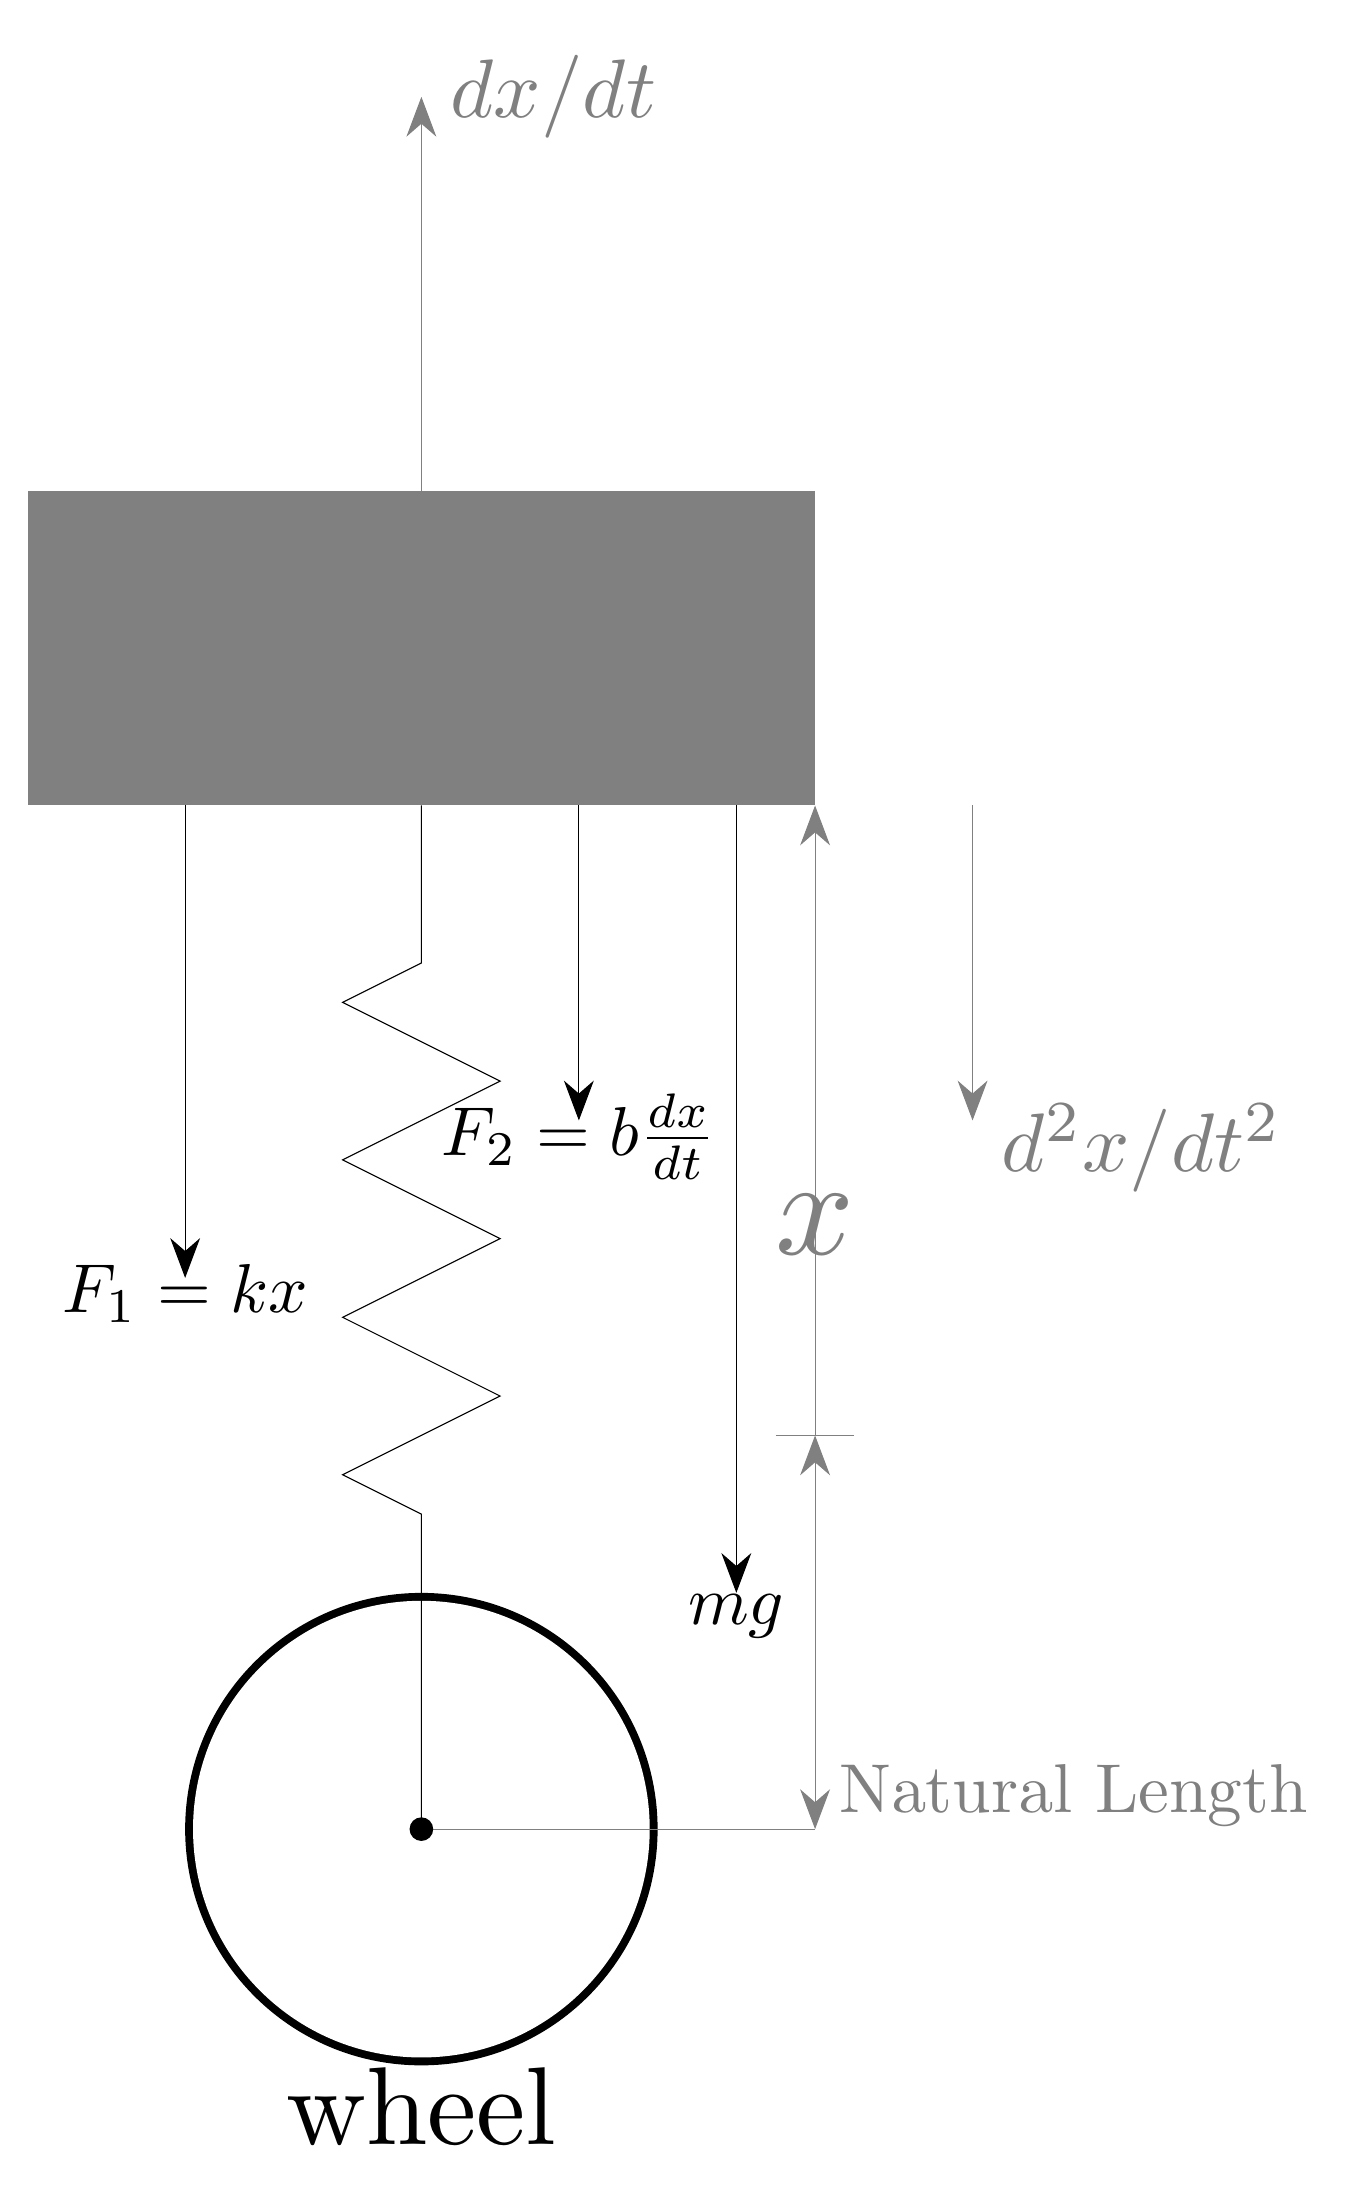
\begin{tikzpicture}
    \fill (5,5) circle [radius=3] node[scale=4,above=-128pt] {wheel};
    \fill[white] (5,5) circle [radius=2.9];
    \draw (5,5) -- (5,9) -- (4,9.5) -- (6,10.5) -- (4,11.5) -- (6,12.5) -- (4,13.5) -- (6,14.5) -- (4,15.5) -- (5,16) -- (5,18);
    \fill[gray] (0,18) rectangle (10,22);
    \draw[gray,-{Stealth[scale=3]}] (10,10) -- (10,18) 
    node[scale=5,above=-180pt] {$x$};
    \draw[gray] (9.5,10) -- (10.5,10);
    \draw[gray,{Stealth[scale=3]}-{Stealth[scale=3]}] (10,5) -- (10,10) node[scale=2.5,above=-130pt,right] {Natural Length};
    \draw[gray] (5,5) -- (10,5);
    \draw[gray,-{Stealth[scale=3]}] (5,22) -- (5,27) node[scale=3][right] {$dx/dt$};
    \draw[-{Stealth[scale=3]}] (2,18) -- (2,12) node[scale=2.5][above=-25pt] {$F_{1}=kx$};
    \draw[-{Stealth[scale=3]}] (7,18) -- (7,14) node[scale=2.5][above=-30pt]{$F_{2}=b\frac{dx}{dt}$};
    \fill (5,5) circle [radius=0.15];
    \draw[gray,-{Stealth[scale=3]}] (12,18) -- (12,14) node[scale=3][above=-10pt, right] {$d^2x/dt^2$};
    \draw[-{Stealth[scale=3]}] (9,18) -- (9,8) node[scale=2.5][above=-25pt] {$mg$};
    
    
\end{tikzpicture}
\end{document}
